\documentclass[11.5pt]{sig-alternate}
\usepackage[defaultlines=3,all]{nowidow}
\usepackage{hyperref}
\usepackage{tabularx}
\usepackage{graphicx}
\usepackage{blindtext}
\usepackage[utf8]{inputenc}
\usepackage[english]{babel}
\usepackage{lastpage}
\usepackage{float}
\usepackage{comment}
\usepackage{multicol}
\usepackage{dirtytalk}
\usepackage{xcolor}
\usepackage{hanging}
\usepackage{array,url,kantlipsum}
\usepackage{wrapfig}
\usepackage[backend=biber, style=apa]{biblatex}
\addbibresource{notation.bib}
\usepackage{authblk}
\usepackage{caption}
\usepackage{graphicx,subfigure}
\usepackage{authblk}
\usepackage{enumitem}
\usepackage[utf8]{inputenc}
\usepackage{cuted}
\usepackage{fancyhdr}
\usepackage{multirow}
\pagestyle{fancy}
\usepackage{lipsum}
\renewcommand{\headrulewidth}{0pt}
\renewcommand{\footrulewidth}{0pt}
\setlength\headheight{80.0pt}
\addtolength{\textheight}{-80.0pt}
\chead{%
  \ifcase\value{page}
  % empty test for page = 0
 \or 
\includegraphics[width=\textwidth]{HTML_JournalBannerIslandConference-02.png}% page=1
  \or 
\includegraphics[width=\textwidth]{HTML_JournalBannerIslandConference-02.png}% page = 2
  \or 
\includegraphics[width=\textwidth]{HTML_JournalBannerIslandConference-02.png}% page = 3
  \or 
\includegraphics[width=\textwidth]{HTML_JournalBannerIslandConference-02.png}% page = 4
  \or 
\includegraphics[width=\textwidth]{HTML_JournalBannerIslandConference-02.png}% page = 5
  \else
  
\includegraphics[width=\textwidth]{HTML_JournalBannerIslandConference-02.png}
  \fi
}

%\chead{
\includegraphics[width=\textwidth]{headerImage.png}}
\fancyfoot[LE,LO]{B/LV Laboratory Accessibility Technology Adapted for Neurodiverse Chemistry Students\\           
DOI: 10.14448/jsesd.15.0004}
\fancyfoot[CE,CO]{{ }}
\fancyfoot[RE,RO]{\thepage}
\pagenumbering{arabic}
\hypersetup{
    colorlinks=true,
    urlcolor=blue
}
 
\let\oldabstract\abstract
\let\oldendabstract\endabstract
\makeatletter
\renewenvironment{abstract}
{\renewenvironment{quotation}%
               {\list{}{\addtolength{\leftmargin}{1em} % change this value to add or remove length to the the default
                        \listparindent 1.5em%
                        \itemindent    \listparindent%
                        \rightmargin   \leftmargin%
                        \parsep        \z@ \@plus\p@}%
                \item\relax}%
               {\endlist}%
\oldabstract}
{\oldendabstract}
\makeatother

% Left align captions
\captionsetup{justification   = raggedright,
              singlelinecheck = false}


\begin{document}

\title{B/LV Laboratory Accessibility Technology Adapted for Neurodiverse Chemistry Students}

\author[1]{\large \color{blue} Christin B. Monroe}



\affil[1]{Landmark College}
\toappear{}

\maketitle
\begin{@twocolumnfalse} 
\begin{abstract}
\item 
\begin{large}
 \textit{Text-to-speech (TTS) technology is a common accommodation available for students with disabilities. Despite the ubiquitous nature of TTS, this technology has not been explored in laboratory settings for neurodiverse college students. This study explores the adaptability of laboratory accessible TTS technology (originally developed for blind/low vision (B/LV) students) for neurodiverse students. Students were asked to provide general feedback about the usability and effectiveness of the technology using Likert surveys. The students also answered open-ended questions about how the technology could be adapted to be more neurodiverse friendly. Overall, more than 50\% of the students found the technology useful but had specific feedback about adaptations that could make it even more universal.}\\
 

   
     
     Keywords: Neurodiversity; Accessible Technology; Chemistry; Text-to-Speech
 \end{large}     
\end{abstract}
\end{@twocolumnfalse}

%% ABSTRACT


%% AUTHOR INFORMATION

\textbf{*Corresponding Author, Christin B. Monroe}\\
\href{mailto: christinmonroe@landmark.edu}{(christinmonroe@landmark.edu)} \\
\textit{Submitted Mon Jan 14, 2023}\\
\textit{Accepted Fri March 31, 2023} \\
\textit{Published online June 15, 2023} \\
\textit{DOI: 10.14448/jsesd.15.0004} \\

\pagebreak
\pagebreak

\vspace{5mm}
\section*{\vspace{140mm}}
\section*{Background}
\subsubsection*{Definition of Neurodiversity}
\begin{large}
Neurodiversity is a social ideal based on a biological fact. The human brain is the most complex
thing on Earth, and every brain is different. Neurodiversity is about what that should mean. Instead of separating people into normal and abnormal, neurodiversity asks us to accept variation. To us, it means that autism, ADHD, and learning disabilities are valuable forms of humanity that enrich culture. New ideas, insights, and unique ways of viewing the world come from diverse minds. This is a strength. (Landmark College Center for Neurodiversity, n.d.)

Neurodiverse students have been historically underrepresented in STEM education at the postsecondary level. (Moon, Utschig, Todd, \& Bozzorg, 2011)  Only 10\% of individuals who report having a disability are awarded science and engineering doctoral degrees and only 5\% of all employed science, engineering and health doctorate holders report having a disability. (National Science Foundation (NSF), 2021)  There are many documented bottlenecks for students with disabilities pursuing degrees in Science, Technology, Engineering and Mathematics \\(STEM). (Friedensen, Lauterbach, Kimball, \& Mwangi, 2021) Assistive technology is an umbrella term that encompasses any technology device, program, website or other resource that enables students with special needs to have fair and appropriate access to curriculum and learning of content. (DaCosta, 2014)    Technological advances in assistive technology have the potential to expand opportunities for students with disabilities, but few studies have explored the use of assistive technology in laboratory settings, especially with neurodiverse students.  Assistive technology has been shown to be beneficial for neurodiverse middle school students learning scientific vocabulary. (Gomes \& Mensah, 2016)

While there is significant potential for the use of assistive technology to expand opportunities for individuals with disabilities in STEM, there are barriers to integrate this technology into classrooms.  These barriers include: 1) expense, 2) lack of time, 3) training, 4) maintenance and responsibility and 5) cultural barriers. (DaCosta, 2014)  During the implementation of assistive technology, training for both instructors and students must be included, along with a clear vision for how the technology can meet the needs of the learner. (Lange, McPhillips, Mulhern, \& Wylie, 2006)  The instructor must also consider the goals of the assignment to identify when to implement the technology.  Ideally, the technology can benefit all learners and can be widely implemented, preventing marginalization and implementation of Universal Design for Learning (UDL) (Tobin \& Behling, 2018).   The technology should also be adapted to meet the needs of varied audiences, as in the case of this study expansion of blind/low vision (B/LV) technology for neurodiverse students who may or may not have vision challenges.

The assistive technology utilized in this study is the Talking Labquest 2 (TLQ).  This technology is an adaptation of the first accessible portable scientific data collection device for students with B/LV. (Supalo, 2013)  The Labquest 2 was first released from Vernier Science Education in 2012 and the display characteristics (along with the touch screen capabilities) are outdated compared to the updated Labquest 3 model and tablet technology.  However, currently the most recent TLQ software is only compatible with Labquest 2 models.  Previous studies with this technology have been shown to foster the development of self-beliefs to independently function in scientific domains. (Isaacson, Michaels, Supalo, \& Roth, 2016)  The benefits of TTS technology for students with language based learning differences (like dyslexia) are well documented, including better  understanding of the text without having to decode the words on the page and prevention of eye strain. (Smythe, 2010)  Not all students benefit from TTS (Silvestri, Holmes, \& Rahemtulla, 2022), but expansion of accessible laboratory technology for neurodiverse individuals has the potential to expand the student and professional STEM workforce.  This study aims to explore whether students with language-based learning differences can benefit from the TTS technology utilized directly within the laboratory setting.

\section*{Methods}
\subsubsection*{Institutional Review Board (IRB)}
All procedures and materials were approved by a college IRB.

\subsubsection*{Participants}
A total of 11 neurodiverse students were asked to provide feedback on their use of the TLQ 2.  All participants were enrolled in an introductory college level chemistry course.  All participants that opted to participate had previously found TTS technology useful in other contexts outside of the laboratory setting.

\subsubsection*{Design}
Students were asked to complete a post survey after working with the TLQ either in the laboratory setting or in a classroom setting.  Students in the laboratory setting were asked to provide feedback on the real time TTS data collection and on the TTS instructions embedded in the TLQ 2 software.  Students in the classroom setting were asked to provide feedback on the TTS on-board periodic table.  

\section*{Materials}
\subsubsection*{Classroom Laboratory Experiments}
Laboratory experiments were selected from the Vernier Software \& Technology Lab Book Advanced Chemistry with Vernier (Vernier Science Education, 2019).

\subsubsection*{Survey Instruments}
Three Likert surveys were utilized to assess the usefulness of the TLQ instrument.  Each survey used the following five point scale: 4= Strongly agree; 3= Agree; 2= Disagree; 1= Strongly Disagree; 0= Neither or N/A.  All surveys can be found in the supplementary materials.  Surveys were designed based upon tools previously utilized with neurodiverse individuals (S. Wallace, personal communication, March 9th, 2021).  Students were also asked open ended questions to solicit feedback on how to make the technology more neurodiverse friendly.  Survey A was used to assess students’ opinions about the TTS real time data collection.  Survey B was used to assess the students’ opinions about the TTS laboratory instructions built into the TLQ 2.  Survey C was used to assess the student’s opinions about the TTS periodic table.

\subsubsection*{Procedure}
Testing consisted of students completing labs from the Vernier catalog for surveys A and B.  Students completed the “Determining the Enthalpy of a Chemical Reaction” using the Vernier Temperature Probe for Survey A and “Acid-Base Titration” using the Vernier pH probe for Survey B.  Feedback reported by students using the TLQ in a prior study (Kroes, Lefler, Schmitt \& Supalo, 2016) was used to design the current experiment, in particular using separate spaces for the students to complete labs to prevent noise interference.  Prior to completing their labs, the teacher provided instructions on how to use the TLQ.   Survey C was used for the periodic table TTS in the classroom format. 

\section*{Results}
Figure 1 summarizes the feedback collected from students from surveys A and B.  The feedback demonstrates that students think that having access to a tool like the TLQ 2 would be helpful for laboratory experiments, as 81\% of the responses reflected either ‘strongly agree’ or ‘agree’.  The feedback also reflects that more than 50\% of students found the tool helpful.  68\% of students who took part in survey C found the idea of the talking periodic table useful, but also had concerns about the voice and voice style.

\begin{figure}[htp]
    \centering
    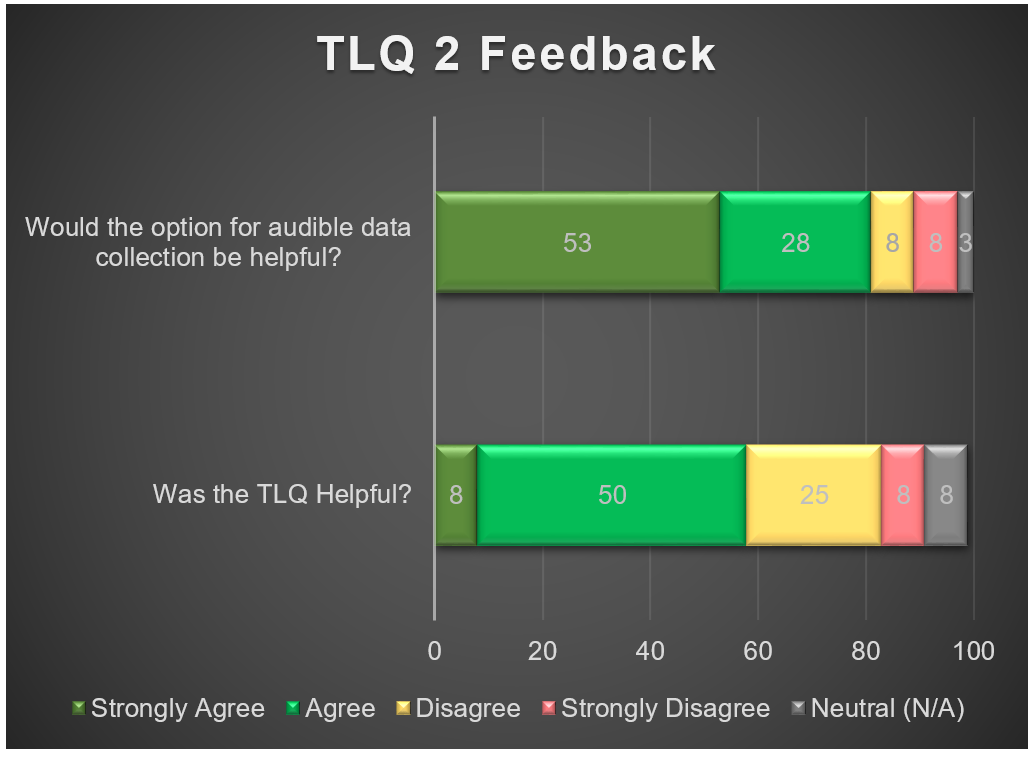
\includegraphics[width=8cm]{figure1.png}
 \caption{Figure summarizing feedback collected from
students using Likert-style questions.}
    \label{Figure summarizing feedback collected from
students using Likert-style questions.}
\end{figure}

Students also articulated that the design of the TLQ 2 (as a tool optimized for blind/ visually impaired (B/VI) individuals) can be adapted to be more versatile for both neurodiverse and neurotypical individuals.  Students felt that the “robotic” voice was difficult to process.  All students that submitted feedback to the open-ended questions made suggestions about embedding options for different TTS voices.  TTS software commonly used by neurodiverse individuals includes Kurzweil 3000 and Natural Reader.  These platforms allow students to modify the voice with over 16 embedded US English voice options and allows students to track text as it is being read allowed.   Students also felt that they would benefit from more updated hardware, as the Labquest 2 was first made commercially available in 2012.  The students also felt that having the option for text to be highlighted as it is read or having the words flow onto the page as they are being read would be beneficial.  Another way to keep track of steps would be to “check off” steps in the device as students move through the experiments.  The audiosonification function tool in the TLQ 2 was not tested with students, mainly because the software lacked visual tracking as the point travels along the graph.

Students also commented on the ability to utilize the TLQ 2 as an “additional lab partner”, which allows them to focus more on the hands-on aspects of learning laboratory techniques.  Taking into consideration cognitive load theory (CLT) (Schnotz \& Kurschner, 2007), implementation of TTS technology has the potential to decrease extraneous load, the processing load caused by the format of the instruction, and maximize intrinsic load.  This would provide students a better opportunity to demonstrate their content knowledge during laboratory experiments.   

\section*{Conclusions}
Based upon the information collected from students in this study, neurodiverse students would likely benefit from having the combination of visual and audio cues, which could be incorporated into future iterations of this technology.  More than 50\% of students found the idea of the TLQ 2 helpful and provided specific suggestions that would expand the versatility of the device, by making it more neurodiverse friendly.  Expansion of accessible science learning devices may increase the number of neurodiverse students and professionals  and increase diversity in STEM fields. (Isaacson, Michaels, Supalo, \& Roth, 2016)  This study demonstrates the potential to expand the versatility of pre-existing B/VI accessible technology to serve another underserved population , neurodiverse students.  

\section*{Acknowledgements}
The author would like to thank Dr. Cary Supalo, Ashley Neybert and Dr. Greg Williams from Independence Science for support with TLQ 2 software. The author would also like to thank Jamie Harvey for his research assistance with this project. The material is based on work supported by the National Science Foundation under Grant No. 2129912 and the 2022 Landmark College Research grant.

\newpage
\section*{Bibliography}\par 

\leftskip 0.25in
\parindent -0.25in 
%%%

DaCosta, B. (Ed.). (2014). Assitive Technology Research, Pratice and Theory. IGI Global.

Friedensen, R., Lauterbach, A., Kimball, E., \& Mwangi, C. G. (2021). Students with High-Incidence Disabilities in STEM: Barriers Encountered in Postsecondary Learning Environments. Journal of Postsecondary Education and Disability, 77-90.

Gomes, C. V., \& Mensah, F. M. (2016). Sounding out science: Using assistive technology for students with learning differences in middle school science classes. In M. J. Urban, \& D. A. Falvo, Improving K-12 STEM Education Outcomes through Technological Integration (pp. 44-67). IGI Global.

Isaacson, M. D., Michaels, M., Supalo, C., \& Roth, A. (2016). An Examination of Accessible Hands-on Science Learning Experiences, Self-confidence in One's Capacity to Function in the Sciences, and Motivation and Interest in Scientific Careers and Studies. Journal of Science Education for Students with Disabilities, 68-75.

Kroes, K., Lefler, D., Schmitt, A., \& Supalo, C. A. (2016). Development of Assessible Laboratory Experiments for Students with Visual Impairments. Journal of Science Education for Students with Disabilities, 61-67.

Landmark College Center for Neurodiversity. (n.d.). Center of Neurodiverstiy. Retrieved from Landmark College: https://www.land\\mark.edu/center-for-neurodiversity

Lange, A. A., McPhillips, M., Mulhern, G., \& Wylie, J. (2006). Assistive Software Tools for Secondary-Level Students with Literacy Difficulties. Journal of Special Education Technology, 13-22.

Moon, N. W., Utschig, T. T., Todd, R. L., \& Bozzorg, A. (2011). Evaluation of Programmatic Interventions to Improve Postsecondary STEM Education for Students with Disabilities: Findings from SciTrain University. Journal of Postsecondary Education and Disability, 331-349.

National Science Foundation (NSF). (2021). \\Women, Minorities, and Persons with Disabilities in Science and Engineering. Alexandria, VA: National Center for Science and Engineering Statistics (NCSES).

Schnotz, W., \& Kurschner, C. (2007). A Reconsideration of Cognitive Load Theory. Educational Psychological Review, 469-507.

Silvestri, R., Holmes, A., \& Rahemtulla, R. (2022). The interaction of cognitive profiles and TTS software on reading comprehension of adolescents with reading challenges. Journal of Special Education Technology , 498-509.

Smythe, I. (2010). Dyslexia in the Digital Age. A\&C Black.

Supalo, C. A. (2013). The Next Generation Laboratory Interface for Students with Blindness or Low Vision in the Science Laboratory. Journal of Science Education for Students with Disabilities. Retrieved from https://scholarworks.rit.edu/jsesd/vol16/iss1/5

Tobin, T. J., \& Behling, K. T. (2018). Reach Everyone, Teach Everyone: Universal Design for Learning in Higher Education. Morgantown: West Virginia University Press.

Vernier Science Education. (2019). Advanced Chemistry with Vernier. Beaverton, OR: Vernier Software \& Technology.

\clearpage

\section*{Supplementary Information}

\begin{table}[h!]
\caption*{Survey A}
\label{tab:Survey A}
\resizebox{\textwidth}{!}{%
\begin{tabular}{cl|c|c|c|c|c|}
\cline{3-7}
\multicolumn{1}{l}{} &
   &
  \multicolumn{1}{l|}{\begin{tabular}[c]{@{}l@{}}Strongly \\ Agree\end{tabular}} &
  \multicolumn{1}{l|}{Agree} &
  \multicolumn{1}{l|}{Disagree} &
  \multicolumn{1}{l|}{\begin{tabular}[c]{@{}l@{}}Strongly \\ Disagree\end{tabular}} &
  \multicolumn{1}{l|}{\begin{tabular}[c]{@{}l@{}}Neither \\or  N/A\end{tabular}} \\ \hline
\multicolumn{1}{|c|}{1.} &
  \begin{tabular}[c]{@{}l@{}}I find it is harder to monitor data collection, \\ if the data is read out to me while it is collected.\end{tabular} &
  4 &
  3 &
  2 &
  1 &
  0 \\ \hline
\multicolumn{1}{|c|}{2.} &
  \begin{tabular}[c]{@{}l@{}}If given a choice, I would prefer to have access \\ to audible versions of the laboratory manual to \\ use while performing a lab.\end{tabular} &
  4 &
  3 &
  2 &
  1 &
  0 \\ \hline
\multicolumn{1}{|c|}{3.} &
  \begin{tabular}[c]{@{}l@{}}I do not feel that I can fully understand data \\ unless it is presented in multiple formats, \\ including visual and auditory.\end{tabular} &
  4 &
  3 &
  2 &
  1 &
  0 \\ \hline
\multicolumn{1}{|c|}{4.} &
  \begin{tabular}[c]{@{}l@{}}If given a choice, I would prefer to have the \\ option to have data read out to me during a \\ laboratory exercise.\end{tabular} &
  4 &
  3 &
  2 &
  1 &
  0 \\ \hline
\multicolumn{1}{|c|}{5.} &
  \begin{tabular}[c]{@{}l@{}}I find that having the option for both audible \\ and visual data collection and analysis helps \\ me to better interpret laboratory data.\end{tabular} &
  4 &
  3 &
  2 &
  1 &
  0 \\ \hline
\multicolumn{1}{|c|}{6.} &
  \begin{tabular}[c]{@{}l@{}}If given a choice, I would prefer only to have \\ data collected as a graph or data table without \\ it being read to me real time.\end{tabular} &
  4 &
  3 &
  2 &
  1 &
  0 \\ \hline
\multicolumn{1}{|c|}{7.} &
  \begin{tabular}[c]{@{}l@{}}Without the aid of the auditory data collection \\ I felt comfortable monitoring and evaluating \\ laboratory experiments.\end{tabular} &
  4 &
  3 &
  2 &
  1 &
  0 \\ \hline
\multicolumn{1}{|c|}{8.} &
  \begin{tabular}[c]{@{}l@{}}Having the Talking LabQuest 2 in the laboratory \\ did not provide any benefit to performing \\ laboratory activities.\end{tabular} &
  4 &
  3 &
  2 &
  1 &
  0 \\ \hline
\multicolumn{1}{|c|}{9.} &
  \begin{tabular}[c]{@{}l@{}}The Talking LabQuest 2 accessories helped me \\ feel more comfortable performing laboratory \\ experiments.\end{tabular} &
  4 &
  3 &
  2 &
  1 &
  0 \\ \hline
\multicolumn{1}{|c|}{10.} &
  \begin{tabular}[c]{@{}l@{}}Before using the Talking LabQuest 2, I felt \\ confident performing laboratory experiments.\end{tabular} &
  4 &
  3 &
  2 &
  1 &
  0 \\ \hline
\multicolumn{1}{|c|}{11.} &
  \begin{tabular}[c]{@{}l@{}}I learn best when I have a variety of stimulations, \\ including (but not limited to) auditory and visual.\end{tabular} &
  4 &
  3 &
  2 &
  1 &
  0 \\ \hline
\multicolumn{1}{|c|}{12.} &
  \begin{tabular}[c]{@{}l@{}}I find I can organize numerical data best when it \\ is read to me.\end{tabular} &
  4 &
  3 &
  2 &
  1 &
  0 \\ \hline
\multicolumn{1}{|c|}{13.} &
  \begin{tabular}[c]{@{}l@{}}Having an audible version of data made it easier \\ to interpret changes happening during the data \\ collection process.\end{tabular} &
  4 &
  3 &
  2 &
  1 &
  0 \\ \hline
\multicolumn{1}{|c|}{14.} &
  \begin{tabular}[c]{@{}l@{}}If given a choice to do a laboratory with the \\ Talking Labquest 2, I would prefer to have \\ access to it.\end{tabular} &
  4 &
  3 &
  2 &
  1 &
  0 \\ \hline
\multicolumn{1}{|c|}{15.} &
  \begin{tabular}[c]{@{}l@{}}If given a choice, I would prefer only to have \\ instructions and data presented in written form.\end{tabular} &
  4 &
  3 &
  2 &
  1 &
  0 \\ \hline
\end{tabular}%
}
\end{table}

\clearpage

\begin{table}[h!]
\caption*{Survey B}
\label{tab:Survey B}
\resizebox{\textwidth}{!}{%
\begin{tabular}{cl|c|c|c|c|c|}
\cline{3-7}
 &
   &
  \multicolumn{1}{l|}{\begin{tabular}[c]{@{}l@{}}Strongly \\ Agree\end{tabular}} &
  \multicolumn{1}{l|}{Agree} &
  \multicolumn{1}{l|}{Disagree} &
  \multicolumn{1}{l|}{\begin{tabular}[c]{@{}l@{}}Strongly \\ Disagree\end{tabular}} &
  \multicolumn{1}{l|}{\begin{tabular}[c]{@{}l@{}}Neither \\or N/A\end{tabular}} \\ \hline
\multicolumn{1}{|c|}{16.} &
  \begin{tabular}[c]{@{}l@{}}Having an audible version of data made it easier to \\ interpret changes happening during the data \\ collection process.\end{tabular} &
  4 &
  3 &
  2 &
  1 &
  0 \\ \hline
\multicolumn{1}{|c|}{17.} &
  \begin{tabular}[c]{@{}l@{}}If given a choice to do a laboratory with the Talking \\ LabQuest 2, I would prefer to have access to it.\end{tabular} &
  4 &
  3 &
  2 &
  1 &
  0 \\ \hline
\multicolumn{1}{|c|}{18.} &
  \begin{tabular}[c]{@{}l@{}}If given a choice, I would prefer only to have \\ instructions and data presented in written form.\end{tabular} &
  4 &
  3 &
  2 &
  1 &
  0 \\ \hline
\multicolumn{1}{|c|}{19.} &
  \begin{tabular}[c]{@{}l@{}}When only provided with a written protocol, I find it \\ is straightforward to complete hands-on labs.\end{tabular} &
  4 &
  3 &
  2 &
  1 &
  0 \\ \hline
\multicolumn{1}{|c|}{20.} &
  \begin{tabular}[c]{@{}l@{}}I find audible instructions easier to follow compared \\ to written instructions.\end{tabular} &
  4 &
  3 &
  2 &
  1 &
  0 \\ \hline
\multicolumn{1}{|c|}{21.} &
  \begin{tabular}[c]{@{}l@{}}If given a choice, I would prefer to have access to \\ audible versions of the laboratory manual to use \\ while performing a lab.\end{tabular} &
  4 &
  3 &
  2 &
  1 &
  0 \\ \hline
\multicolumn{1}{|c|}{22.} &
  \begin{tabular}[c]{@{}l@{}}Having a solely written protocol in front of me is \\ enough for me to comfortably complete a \\ laboratory assignment.\end{tabular} &
  4 &
  3 &
  2 &
  1 &
  0 \\ \hline
\multicolumn{1}{|c|}{23.} &
  \begin{tabular}[c]{@{}l@{}}Without the aid of the audible laboratory lab \\ manual I felt comfortable performing \\ laboratory experiments.\end{tabular} &
  4 &
  3 &
  2 &
  1 &
  0 \\ \hline
\multicolumn{1}{|c|}{24.} &
  \begin{tabular}[c]{@{}l@{}}If given a choice, I would prefer only to have \\ instructions and data presented in written form.\end{tabular} &
  4 &
  3 &
  2 &
  1 &
  0 \\ \hline
\end{tabular}%
}
\end{table}


Open Ended Survey Questions:
\begin{enumerate}
    \item What can be done to improve the technology?
    \item What can be done to make the procedure for the technology more understandable?
    \item Was the overview of the technology in the beginning useful?
    \item Should we overview any other features that you would have liked to use?
    \item Are there any features you would have liked to have the technology do during this lab that it does not already do?
\end{enumerate}


\clearpage


\begin{table}[h!]
\caption*{Survey C}
\label{tab:Survey C}
\resizebox{\textwidth}{!}{%
\begin{tabular}{cl|c|c|c|c|c|}
\cline{3-7}
 &
   &
  \multicolumn{1}{l|}{\begin{tabular}[c]{@{}l@{}}Strongly \\ Agree\end{tabular}} &
  \multicolumn{1}{l|}{Agree} &
  \multicolumn{1}{l|}{Disagree} &
  \multicolumn{1}{l|}{\begin{tabular}[c]{@{}l@{}}Strongly \\ Disagree\end{tabular}} &
  \multicolumn{1}{l|}{\begin{tabular}[c]{@{}l@{}}Neither \\ or N/A\end{tabular}} \\ \hline
\multicolumn{1}{|c|}{25.} &
  \begin{tabular}[c]{@{}l@{}}If given a choice, I would prefer to have the option to \\ have data read out to me during a laboratory exercise.\end{tabular} &
  4 &
  3 &
  2 &
  1 &
  0 \\ \hline
\multicolumn{1}{|c|}{26.} &
  \begin{tabular}[c]{@{}l@{}}If given a choice, I would prefer only to have data \\ collected as a graph or data table without it being \\ read to me real time.\end{tabular} &
  4 &
  3 &
  2 &
  1 &
  0 \\ \hline
\multicolumn{1}{|c|}{27.} &
  \begin{tabular}[c]{@{}l@{}}I feel comfortable accessing information from the \\ periodic table, without the use of auditory options.\end{tabular} &
  4 &
  3 &
  2 &
  1 &
  0 \\ \hline
\multicolumn{1}{|c|}{28.} &
  \begin{tabular}[c]{@{}l@{}}I learned best when I have a variety of stimulations, \\ including (but not limited to) auditory and visual.\end{tabular} &
  4 &
  3 &
  2 &
  1 &
  0 \\ \hline
\multicolumn{1}{|c|}{29.} &
  \begin{tabular}[c]{@{}l@{}}I find I can organize numerical data best when it \\ is read to me.\end{tabular} &
  4 &
  3 &
  2 &
  1 &
  0 \\ \hline
\multicolumn{1}{|c|}{30.} &
  \begin{tabular}[c]{@{}l@{}}After using the accessible periodic table, I felt \\ more comfortable extracting information from \\ the periodic table.\end{tabular} &
  4 &
  3 &
  2 &
  1 &
  0 \\ \hline
\multicolumn{1}{|c|}{31.} &
  \begin{tabular}[c]{@{}l@{}}If given a choice to do a laboratory with the \\ Talking LabQuest 2, I would prefer to have \\ access to it.\end{tabular} &
  4 &
  3 &
  2 &
  1 &
  0 \\ \hline
\multicolumn{1}{|c|}{32.} &
  \begin{tabular}[c]{@{}l@{}}If given a choice, I would prefer only to have \\ instructions and data presented in written form.\end{tabular} &
  4 &
  3 &
  2 &
  1 &
  0 \\ \hline
\end{tabular}%
}
\end{table}

\end{large}
\end{document}
